\begin{figure*}[t]
	\addtolength{\tabcolsep}{-4.5pt}
	\begin{tabular}{ccccccccc}
		& \multicolumn{2}{c}{\toptext{2\resultwidth}{Point estimate}} & \multicolumn{5}{c}{\toptext{5\resultwidth}{Bayesian inference}}\\[-4pt]
		target & loss & optimize & posterior & sample-1 & sample-2 & sample-3& sample-4
		\\
		
\includegraphics[width=\resultwidth]{images/synth/bump/out/target.jpg} &
		\includegraphics[width=\resultwidth]{images/synth/bump/out/loss.pdf} &
		\includegraphics[width=\resultwidth]{images/synth/bump/out/optim.jpg} &
		\includegraphics[width=\resultwidth]{images/synth/bump/out/posterior.pdf} &
		\includegraphics[width=\resultwidth]{images/synth/bump/out/good1.jpg} &
		\includegraphics[width=\resultwidth]{images/synth/bump/out/good2.jpg} &
		\includegraphics[width=\resultwidth]{images/synth/bump/out/good3.jpg} &
		\includegraphics[width=\resultwidth]{images/synth/bump/out/bad1.jpg}
		\\
		
\includegraphics[width=\resultwidth]{images/synth/leather/out/target.jpg} &
		\includegraphics[width=\resultwidth]{images/synth/leather/out/loss.pdf} &
		\includegraphics[width=\resultwidth]{images/synth/leather/out/optim.jpg} &
		\includegraphics[width=\resultwidth]{images/synth/leather/out/posterior.pdf} &
		\includegraphics[width=\resultwidth]{images/synth/leather/out/good1.jpg} &
		\includegraphics[width=\resultwidth]{images/synth/leather/out/good2.jpg} &
		\includegraphics[width=\resultwidth]{images/synth/leather/out/good3.jpg} &
		\includegraphics[width=\resultwidth]{images/synth/leather/out/bad1.jpg}
		\\
		
\includegraphics[width=\resultwidth]{images/synth/plaster/out/target.jpg} &
		\includegraphics[width=\resultwidth]{images/synth/plaster/out/loss.pdf} &
		\includegraphics[width=\resultwidth]{images/synth/plaster/out/optim.jpg} &
		\includegraphics[width=\resultwidth]{images/synth/plaster/out/posterior.pdf} &
		\includegraphics[width=\resultwidth]{images/synth/plaster/out/good1.jpg} &
		\includegraphics[width=\resultwidth]{images/synth/plaster/out/good2.jpg} &
		\includegraphics[width=\resultwidth]{images/synth/plaster/out/good3.jpg} &
		\includegraphics[width=\resultwidth]{images/synth/plaster/out/bad1.jpg}
		\\
		
\includegraphics[width=\resultwidth]{images/synth/flake/out/target.jpg} &
		\includegraphics[width=\resultwidth]{images/synth/flake/out/loss.pdf} &
		\includegraphics[width=\resultwidth]{images/synth/flake/out/optim.jpg} &
		\includegraphics[width=\resultwidth]{images/synth/flake/out/posterior.pdf} &
		\includegraphics[width=\resultwidth]{images/synth/flake/out/good1.jpg} &
		\includegraphics[width=\resultwidth]{images/synth/flake/out/good2.jpg} &
		\includegraphics[width=\resultwidth]{images/synth/flake/out/good3.jpg} &
		\includegraphics[width=\resultwidth]{images/synth/flake/out/bad1.jpg}
		\\
		
\includegraphics[width=\resultwidth]{images/synth/metal/out/target.jpg} &
		\includegraphics[width=\resultwidth]{images/synth/metal/out/loss.pdf} &
		\includegraphics[width=\resultwidth]{images/synth/metal/out/optim.jpg} &
		\includegraphics[width=\resultwidth]{images/synth/metal/out/posterior.pdf} &
		\includegraphics[width=\resultwidth]{images/synth/metal/out/good1.jpg} &
		\includegraphics[width=\resultwidth]{images/synth/metal/out/good2.jpg} &
		\includegraphics[width=\resultwidth]{images/synth/metal/out/good3.jpg} &
		\includegraphics[width=\resultwidth]{images/synth/metal/out/bad1.jpg}
		\\
		
\includegraphics[width=\resultwidth]{images/synth/wood/out/target.jpg} &
		\includegraphics[width=\resultwidth]{images/synth/wood/out/loss.pdf} &
		\includegraphics[width=\resultwidth]{images/synth/wood/out/optim.jpg} &
		\includegraphics[width=\resultwidth]{images/synth/wood/out/posterior.pdf} &
		\includegraphics[width=\resultwidth]{images/synth/wood/out/good1.jpg} &
		\includegraphics[width=\resultwidth]{images/synth/wood/out/good2.jpg} &
		\includegraphics[width=\resultwidth]{images/synth/wood/out/good3.jpg} &
		\includegraphics[width=\resultwidth]{images/synth/wood/out/bad1.jpg}
		\\
		& & \qquad \qquad \, low &
		\includegraphics[width=\resultwidthpdf]{images/img/colorbar.png} &
		high \qquad \qquad \,& & &
	\end{tabular}
	%
	\caption{\label{fig:synth}
		\textbf{Optimization and HMC sampling on synthetic images.} Each row corresponds to a different material. From top: bump, leather, plaster, metallic flake, brushed metal and wood. Column 1 is rendered images using different forward models. We show optimization results in columns 2 and 3, samplings in the rest columns. For high dimensional posterior visualization, we project them to 2D using PCA. Here we only show the first two major components. The three red dots corresponding to sample-1,2,3, which are closer to the peak of high dimensional distribution. and the green dot (sample-4) is the opposite. More results please refer to supplemental materials.
	}
\end{figure*}

